\nocite{04d6b664}
\nocite{6ab9663f}
\nocite{f6db8935}
\nocite{fa76af21}
In this section we want to shift our focus to a more quantitative understanding of topological insulators after our qualitative presentation in section \ref{sec:topins}. For that purpose we study a certain model of a certain topological insualtor due to Kane and Mele. They described a model of a two-dimensional topological insulator with Cartan label AII and a formula to compute the according topological invariant. Our goal is to portray their paper \cite{04d6b664} in the context of section \ref{sec:topins} enhancing our understanding of topological insulators by a more detailed example. As a result we will first describe the Kane-Mele model as an insulator comprising a crystal structure, a Hamiltonian and its direct integral decomposition followed by a discussion of the topological invariant. By going to a lower level than before we can relate it to the IQHE and identify it as the \textit{quantum spin Hall effect (QSHE)} which got its name from its origin in the electron spin.
\\
So first let us have a look at the crystal structure of the Kane-Mele model. It is a {\glqq}honey comb{\grqq} structure.\footnote{if you don't believe you can draw it} Formally, let $d \in (0,\infty)$ and
\begin{align*}
  d_{1}
  :=
  d
  \left(
    \frac{1}{2},
    -\frac{\sqrt{3}}{2}
  \right)
  \in
  \mathbb{R}^{2}
  &&
  d_{2}
  :=
  d
  \left(
    \frac{1}{2},
    \frac{\sqrt{3}}{2}
  \right)
  \in
  \mathbb{R}^{2}
  &&
  d_{3}
  :=
  -
  (d_{1} + d_{2})
\end{align*}
Let further
\begin{align*}
  l_{1}
  :=
  d_{2}
  -
  d_{3}
  &&
  l_{2}
  :=
  d_{3}
  -
  d_{1}
  &&
  l_{3}
  :=
  -
  (l_{1}+l_{2})
\end{align*}
Then $L_{\textrm{km}} := \mathrm{span}_{\mathbb{Z}}(l_{1},l_{2})$ is the Kane-Mele model's lattice. Next, the c-basis: Here we choose $\mathfrak{C}_{\textrm{km}} := \lbrace 0,d_{2} \rbrace$ and $\mathsf{A}_{\textrm{km}} := \lbrace A,B \rbrace$ together with the function $f_{\textrm{km}} := \lbrace (0,A),(d_{2},B) \rbrace \subset \mathfrak{C}_{\textrm{km}} \times \mathsf{A}_{\textrm{km}}$. The explicit sort of atomic nuclei is not relevant for our theoretical considerations.
\\
After having specified the crystal structure of the Kane-Mele model we need the Hamilton operator that describes the physics. Since the Hamilton operator $H = H_{0} + M_{V}$ from section \ref{sec:topins} where $H_{0}$ is the one with the pauli matrices is too complicated one puts a {\glqq}tight binding approximation{\grqq} to work together with some correction terms making it sufficiently close to what one had in mind originally. Descriptively, tight binding means that the electrons are narrowly located around a crystal site and therefore are not feeling the potential generated by the other sites. To use this approximation here is physically vindicated by the observation that the framework using lattices from \ref{sec:topins} is in general only valid for temperatures near zero and thus the electrons occupy the lowest energy levels. In other words, they are probably close to an atomic nucleus. So in the tight binding approximation the crystal sites are assumed to be isolated quantum systems, that is, one Hamilton operator per crystal site/atomic nucleus. As usual, one models an atomic nucleus as a Coulomb-like system. Then, after solving the Schroedinger equation for all those Coulomb-like systems possibly subjected to a magnetic field, we get annihilation operators
\begin{align*}
  c_{(l,c)}
  &=
  (c_{(l,c)}^{\uparrow},c_{(l.c)}^{\downarrow})
\end{align*}
with two components due to spin $1/2$ for every crystal site \begin{align*}
  (l,c)
  \in
  L_{\textrm{km}}
  \times
  \mathfrak{C}_{\textrm{km}}
  &=:
  \mathrm{C}_{\textrm{km}}
\end{align*}
Being an \textit{annihilation operator} means that for a given eigenvector $\psi_{n}$ of the Hamilton operator - please note the pure point spectrum - to the eigenvalue $E_{n}$ where $n \in \mathbb{N}$ the vector $c_{(l,c)}(\psi_{n})$ is an eigenvector to the eigenvalue $E_{n-1}$ if $n > 0$ and $0$ else. The adjoint $c_{(l,c)}^{\ast}$ of $c_{(l,c)}$ is called \textit{creation operator} and does the obvious. In \textit{second quantization} tight binding then means \textit{nearest neighbor hopping}. Two crystal sites are \textit{nearest neighbors} if their distance is $\Vert d_{2} \Vert$. And nearest neighbor hopping means that the annihilation of an electron at a site must result in the creation of an electron at a nearest neighbor site. Let $\textrm{nn}_{(l,c)} \subset \mathrm{C}_{\textrm{km}}$ be the set of nearest neighbors to the crystal site $(l,c) \in \mathrm{C}_{\textrm{km}}$. Then the tight binding Hamilton operator is
\begin{align*}
  H_{\textrm{nn}}
  &:=
  \lambda_{\textrm{nn}}
  \sum_{\langle i,j \rangle}
  c_{j}^{\ast}
  c_{i}
  :=
  \lambda_{\textrm{nn}}
  \sum_{i \in \mathbf{C}_{\textrm{km}}}
  \sum_{j \in \textrm{nn}_{i}}
  \langle
    c_{j}^{\ast},c_{i}
  \rangle
\end{align*}
for $\lambda_{\textrm{nn}} \in \mathbb{R}$ and $\langle \cdot,\cdot \rangle$ the canonical dual pairing. We take three corrections to this model $H_{nn}$ into account to obtain the Kane-Mele model $H_{\textrm{km}}$:
\begin{enumerate}
\item[(SE)]
  The first correction to the tight binding approximation for the Kane-Mele model is the self-energy term. Its physical origin is that two adjacent sites are a priori not equivalent. In second quantization we get
\begin{align*}
  H_{\textrm{se}}
  &:=
  \lambda_{\textrm{se}}
  \sum_{l \in L_{\textrm{km}}}
  \left(
    c_{(l,0)}^{\ast}
    c_{(l,0)}
    -
    c_{(l,d_{2})}^{\ast}
    c_{(l,d_{2})}
  \right)
\end{align*}
for $\lambda_{\textrm{se}} \in \mathbb{R}$.
\item[(SO)]
  The second correction term is spin-orbit coupling originating from the electron spin in the magnetic field generated by the electron momentum and the electric field of the atomic nuclei. First st note that that two crystal sites are \textit{next nearest neighbors} if their distance is $\Vert l_{1} \Vert$. Let $\textrm{nnn}_{(l,c)} \subset \mathrm{C}_{\textrm{km}}$ be the set of next nearest neighbors to the crystal site $(l,c) \in \mathrm{C}_{\textrm{km}}$. Then the spin-orbit term is:
\begin{align*}
  H_{\textrm{so}}
  &:=
  \mathrm{i}
  \lambda_{\textrm{so}}
  \sum_{\langle\langle i,j \rangle\rangle}
  \nu_{ij}
  c_{j}^{\ast}
  \sigma_{3}
  c_{i}
  :=
  \mathrm{i}
  \lambda_{\textrm{so}}
  \sum_{i \in \mathbf{C}_{\textrm{km}}}
  \sum_{j \in \textrm{nnn}_{i}}
  \nu_{ij}
  c_{j}^{\ast}
  \sigma_{3}
  c_{i}
\end{align*}
for $\lambda_{\textrm{so}} \in \mathbb{R}$ and
\begin{align*}
  \nu_{ij}
  &:=
  \frac{2}{\sqrt{3}\Vert d_{2} \Vert^{2}}
  \left(
    (D_{i} \vert e_{1})
    (D_{j} \vert e_{2})
    -
    (D_{i} \vert e_{2})
    (D_{j} \vert e_{1})
  \right)
  =
  \pm
  1
\end{align*}
where $D_{i},D_{j} \in \lbrace \pm d_{1},\pm d_{2},\pm d_{3} \rbrace$ such that $D_{i} + D_{j}$ is the vector connecting next nearest neighbor crystal sites $i,j$.
\item[(RA)]
The third - and last - correction in the Kane-Mele model is a Rashba term. The physical origin is an electric field in $e_{3}$ direction. This can be the result of a substrate carrying the two dimensional layer, for example. But also an external interference is imaginable. However, again a spin-orbit coupling yields
\begin{align*}
  H_{\textrm{ra}}
  &:=
  \mathrm{i}
  \lambda_{\textrm{ra}}
  \sum_{\langle i,j \rangle}
  c_{j}^{\ast}
  ((D_{ij}\vert e_{2})\sigma_{1} - (D_{ij} \vert e_{1})\sigma_{2})
  c_{i}
\end{align*}
for $\lambda_{\textrm{ra}} \in \mathbb{R}$ and $\Vert d_{2} \Vert D_{ij} \in \lbrace \pm d_{1},\pm d_{2},\pm d_{3} \rbrace$ being the vector connecting nearest neighbor sites $i,j$.
\end{enumerate}
On the whole, the Kane-Mele Hamilton operator
\begin{align*}
  H_{\textrm{km}}
  &:=
  H_{\textrm{nn}}
  +
  H_{\textrm{se}}
  +
  H_{\textrm{so}}
  +
  H_{\textrm{ra}}
\end{align*}
approximates the {\glqq}reality{\grqq} sufficiently well here. Even the further simplification of the operator to have domain only $\ell^{2}(\mathrm{C}_{\textrm{km}},\mathbb{C}) \times \mathbb{C}^{2}$ is enough for our purposes. The physical justification is that at zero temperature the bands are fully filled up to the valence band. The \textbf{valence band} is the first band below the Fermi level. An additional electron is then {\glqq}hopping{\grqq} from the lowest energy state above the Fermi level of an atomic nucleus to the lowest state above the Fermi level of a nearest neighbor. So the electronically interesting physics happens around the Fermi level and only one state per nucleus needs to be considered. This is reflected by $\ell^{2}(\mathrm{C}_{\textrm{km}},\mathbb{C}) \times \mathbb{C}^{2}$ when taking into account the possibly lifted spin degeneracy due to magnetic fields. Now states being in $\ell^{2}(\mathrm{C}_{\textrm{km}},\mathbb{C}) \times \mathbb{C}^{2}$ allows translating compositions of creation and annihilation operators to translation operators. Since nearest neighbors $i,j$ are connected by some $\pm d_{k}$ for $k = 1,2,3$ we replace $c_{j}^{\ast}c_{i}$ by a translation operator $(T_{\pm d_{k}})$ defined by
\begin{align*}
  T_{d_{k}}(\psi)(l,c)
  &:=
  \begin{cases}
    \psi(l - d_{k} + d_{2},0)
    &
    c
    =
    d_{2}
    \\
    0
    &
    \text{else}
  \end{cases}
\end{align*}
and $T_{-d_{k}} := T_{d_{k}}^{\ast}$. It is now apparent what $T_{l_{k}}$ is. Using the same symbols for the Hamilton operators we get
\begin{align*}
  H_{\textrm{nn}}
  &=
  \lambda_{\textrm{nn}}
  \sum_{k=1}^{3}
  \left(
    T_{d_{k}}
    +
    T_{-d_{k}}
  \right)
  \otimes
  1_{\mathbb{C}^{2}}
  \\
  H_{\textrm{se}}
  &=
  \lambda_{\textrm{se}}
  (\chi_{A} - \chi_{B})
  1_{\ell^{2}(\mathrm{C}_{\textrm{km}},\mathbb{C})}
  \otimes
  1_{\mathbb{C}^{2}}
  \\
  H_{\textrm{so}}
  &=
  -
  \mathrm{i}
  \lambda_{\textrm{so}}
  (\chi_{A} - \chi_{B})
  \sum_{k=1}^{3}
  \left(
    T_{l_{k}}
    -
    T_{-l_{k}}
  \right)
  \\
  H_{\textrm{ra}}
  &=
  \mathrm{i}
  \lambda_{\textrm{ra}}
  \left(
    \left(
      T_{d_{1}}
      -
      T_{-d_{1}}
    \right)
    \otimes
    \left(
      -
      \frac{\sqrt{3}\sigma_{1} + \sigma_{2}}{2}
    \right)
    +
    \left(
      T_{d_{2}}
      -
      T_{-d_{2}}
    \right)
    \otimes
    \left(
      \frac{\sqrt{3}\sigma_{1} + \sigma_{2}}{2}
    \right)
    +
    \left(
      T_{d_{3}}
      -
      T_{-d_{3}}
    \right)
    \otimes
    \sigma_{2}
  \right)
\end{align*}
where $\chi_{A}(\psi((l,c))) = 1$ if $(c,A) \in f_{\textrm{km}}$ and similar $\chi_{B}$. $H_{\textrm{km}}$ in this shape is the Hamiltonian we will work with. 
\\
Having a Hamiltonian $H_{\textrm{km}}$ we are again interested in a decomposition according to the crystal momentum like that section \ref{sec:topins} to reveal topological information. There is a modified Bloch-Floquet transform that can be defined in pretty much the same way as in section \ref{sec:topins}. But we want to use the usual Bloch-Floquet transform here, since then $\tilde{H}$ has the periodicity of the reciprocal lattice. The Bloch-Floquet transform is unitarily equivalent to the modified one. So the former one is as appropriate as the latter one. The perk of the modified one is that $\tilde{H}(k)$'s domain does not depend on $k$ what makes it very convenient for mathematical considerations. Anyway, the \textbf{Bloch-Floquet transformation} on $\ell^{2}(\mathrm{C}_{\textrm{km}}) \times \mathbb{C}^{2}$ is defined by
\begin{align*}
  \mathcal{B}
  &\colon
  \ell^{2}(\mathrm{C}_{\textrm{km}})
  \times
  \mathbb{C}^{2}
  \to
  L_{2}
  \left(
    B_{L_{\textrm{km}}},
    \ell^{2}(\mathfrak{C}_{\textrm{km}}) 
    \times
    \mathbb{C}^{2}
  \right)
  ,\qquad
  f
  \mapsto
  (\mathcal{B}(f))(k)
  :=
  \sum_{l \in L_{\textrm{km}}}
  \exp(\mathrm{i}(k \vert l))
  f(\cdot - l)
\end{align*}
We see that this depends on the choice of the c-basis. This is the price for the periodicity of $\tilde{H}$. Now for the direct integral decompostion we get
\begin{align*}
  \tilde{H}_{\textrm{nn}}(k)
  &=
  \lambda_{\textrm{nn}}
  \left(
    \left(
      1
      +
      \cos((k \vert l_{1}))
      +
      \cos((k \vert l_{3}))
    \right)
    \sigma_{1}
    \otimes
    1_{\mathbb{C}^{2}}
    +
    \left(
      \sin((k \vert l_{1}))
      -
      \sin((k \vert l_{3}))
    \right)
    \sigma_{2}
    \otimes
    1_{\mathbb{C}^{2}}
  \right)
  \\
  \tilde{H}_{\textrm{se}}(k)
  &=
  \lambda_{\textrm{se}}
  \sigma_{3}
  \otimes
  1_{\mathbb{C}^{2}}
  \\
  \tilde{H}_{\textrm{so}}(k)
  &=
  -
  2
  \lambda_{\textrm{so}}
  \sum_{k=1}^{3}
  \sin((k \vert l_{k}))
  \sigma_{3}
  \otimes
  \sigma_{3}
  \\
  \tilde{H}_{\textrm{ra}}(k)
  &=
  \lambda_{\textrm{ra}}
  \left(
    \frac{\sqrt{3}}{2}
    \left(
      1
      -
      \cos((k \vert l_{3}))
    \right)
    \sigma_{2}
    \otimes
    \sigma_{1}
    +
    \left(
      \cos((k \vert l_{1}))
      -
      \frac{1}{2}
      \left(
        1
        +
        \cos((k \vert l_{3}))
      \right)
    \right)
    \sigma_{2}
    \otimes
    \sigma_{2}
  \right.
  \\
  &\phantom{=}
  \left.
    -
    \frac{\sqrt{3}}{2}
    \sin((k \vert l_{3}))
    \sigma_{1}
    \otimes
    \sigma_{1}
    -
    \left(
      \sin((k \vert l_{1}))
      +
      \frac{1}{2}
      \sin((k \vert l_{3}))
    \right)
    \sigma_{1}
    \otimes
    \sigma_{2}
  \right)
\end{align*}
Due to the linearity of the Bloch-Floquet transformation
\begin{align*}
  \tilde{H}_{\textrm{km}}(k)
  &=
  \tilde{H}_{\textrm{nn}}(k)
  +
  \tilde{H}_{\textrm{se}}(k)
  +
  \tilde{H}_{\textrm{so}}(k)
  +
  \tilde{H}_{\textrm{ra}}(k)
\end{align*}  
holds. Again, the family $\lbrace \tilde{P}_{\textrm{km}}^{I}(k) \colon k \in B_{L_{\textrm{km}}} \rbrace$ is identified with a complex vector bundle.
\\
We claimed that the Kane-Mele model has Cartan label AII. Therefore it should have a time reversal symmetry and no charge conjungation symmetry or combination of both. While we will not argue for the lack of the latter we will sketch how to show the former. For that purpose note that on $\ell^{2}(\mathrm{C}_{\textrm{km}},\mathbb{C}) \times \mathbb{C}^{2}$ a time reversal operator from Wigner's theorem is
\begin{align*}
  \Theta
  &:=
  \left(
    1_{\ell^{2}(\mathrm{C}_{\textrm{km}},\mathbb{C})}
    \otimes
    \sigma_{2}
  \right)
  \circ
  \kappa
\end{align*}
where $\kappa$ means complex conjungation. It is easy to see that applying $\Theta$ twice just changes the sign. Further it is clear that $\Theta$ is an antiunitary operator as composition of a unitary operator and complex conjungation. Hence for all $\psi,\hat{\psi} \in \ell^{2}(\mathrm{C}_{\textrm{km}},\mathbb{C}) \times \mathbb{C}^{2}$
\begin{align*}
  (\Theta(\psi) \vert \Theta(\hat{\psi}))
  &=
(\hat{\psi} \vert \psi)\end{align*}
holds. This in turn immediately yields for all $\psi,\hat{\psi} \in \ell^{2}(\mathrm{C}_{\textrm{km}},\mathbb{C}) \times \mathbb{C}^{2}$
\begin{align*}
  (\Theta(\psi) \vert \hat{\psi})
  &=
  (\Theta(\hat{\psi}) \vert \Theta(\Theta(\psi)))
  =
  -
  (\Theta(\hat{\psi}) \vert \psi)
\end{align*}
and we conclude for all $\psi \in \ell^{2}(\mathrm{C}_{\textrm{km}},\mathbb{C}) \times \mathbb{C}^{2}$
\begin{align*}
  (\Theta(\psi) \vert \psi)
  &=
  0
\end{align*}
from the case $\psi = \hat{\psi}$. If we Bloch-Floquet transform $\Theta$ by $\mathcal{B}\Theta\mathcal{B}^{-1} =: \tilde{\Theta}$ then $\tilde{\Theta}$ is given by
\begin{align*}
  \tilde{\Theta}(\psi)(-k)
  &:=
  \left(
    \left(
      1_{\mathbb{C}^{2}}
      \otimes
      \sigma_{2}
    \right)
    \circ
    \kappa
  \right)
  (\psi(k))
\end{align*}
for $\psi \in  L_{2}(B_{L_{\textrm{km}}},\ell^{2}(\mathfrak{C}_{\textrm{km}}) \times \mathbb{C}^{2})$. In particular, applying $\tilde{\Theta}$ twice just changes the sign yet again. Moreover, there is an equivalence
\begin{align*}
  \Theta
  \circ
  H_{\textrm{km}}
  \circ
  \Theta^{-1}
  =
  H_{\textrm{km}}
  \qquad
  &\Leftrightarrow
  \qquad
  \forall
  [k]
  \in
  \mathbb{R}^{2}/L_{\textrm{km}}^{\prime}
  \quad
  \tilde{\Theta}
  \circ
  \tilde{H}_{\textrm{km}}(k)
  \circ
  \tilde{\Theta}^{-1}
  =
  \tilde{H}_{\textrm{km}}(-k)
\end{align*}
The latter proposition can explicitly be verified from what we have said about $\Theta$ and the equivalence hence shows that $H_{\textrm{km}}$ has a time reversal symmetry.
\\
With the time reversal symmetry in place we are in the position to derive an easy to calculate formula determining the topological phase. To this end let $\psi_{0}(k),\psi_{1}(k)$ denote the eigenvectors to the lowest eigenvalues $E_{0}(k),E_{1}(k)$ of $\tilde{H}_{\textrm{km}}(k)$. Moreover note that there is $[k] \in \mathbb{R}^{2}/L_{\textrm{km}}^{\prime}$ such that
\begin{align*}
  \tilde{H}_{\textrm{km}}(-k)
  &=
  \tilde{\Theta}
  \circ
  \tilde{H}_{\textrm{km}}(k)
  \circ
  \tilde{\Theta}^{-1}
  =
  \tilde{H}_{\textrm{km}}(k)
\end{align*}
$[k] = [0]$ is one example. But also $[k] = [\frac{1}{2}l_{1,2}^{\prime}]$ and $[k] = [\frac{1}{2}(l_{1}^{\prime} + l_{2}^{\prime})]$ have the property as can be directly seen from the shape of $\tilde{H}_{\textrm{km}}$ above and the periodicity of $\sin(\cdot),\cos(\cdot)$. We call the subspace of those points $\mathtt{Ev}$. The subspace containing the points $[k]$ for which
\begin{align*}
  (\psi_{i}(k) \vert \tilde{\Theta}(\psi_{j})(-k))
  &=
  0
\end{align*}
for all $i,j = 0,1$ is called $\mathtt{Odd}$. Note that for $i = j$ this equality is always true due to the antiunitarity of $(1_{\mathbb{C}^{2}} \otimes \sigma_{2}) \circ \kappa$. In particular, $\psi_{i}(k)$ and $\tilde{\Theta}(\psi_{i})(k)$ are linearly independent. For $[k] \in \mathtt{Ev}$ it is apparent that $\tilde{\Theta}(\psi_{0})(k)$ is also an eigenvector to the same eigenvalue as $\psi_{0}(k)$ for $\tilde{H}_{\textrm{km}}(k)$ since $\tilde{H}_{\textrm{km}}(k)$ commutes with $\tilde{\Theta}$. Thus for $[k] \in \mathtt{Ev}$ we can choose
\begin{align*}
  \psi_{1}(k)
  &=
  \tilde{\Theta}(\psi_{0})(k)
\end{align*}
In any case, defining
\begin{align*}
  \mathrm{pf}(k)
  &:=
  (\psi_{0}(k) \vert \tilde{\Theta}(\psi_{1})(k))
\end{align*}
it is clear that
\begin{align*}
  \vert
    \mathrm{pf}(k)
  \vert
  &=
  \begin{cases}
    1
    & 
    [k] \in \mathtt{Ev}
    \\
    0
    &
    [k] \in \mathtt{Odd}
  \end{cases}
\end{align*}
If $[k]$ is in $\mathtt{Odd}$ so is $[-k]$. The topological phase is now determined by the number of pairs $([k],[-k]) \in \mathtt{Odd} \times \mathtt{Odd}$ modulo $2$ where an even number is the ordinary insulating phase. This quantity can be calculated with the help of a winding number
\begin{align*}
  I_{\textrm{km}}
  &:=
  \left(
    \lim_{\delta \downarrow 0}
    \frac{1}{2\pi\mathrm{i}}
    \oint_{\gamma}
    \nabla_{k}
    \ln(\mathrm{pf} + \mathrm{i}\delta)
    \mathrm{d}k
  \right)
  \mod
  2
  \in
  K_{\mathbb{R}}^{-2}(\lbrace x_{0} \rbrace)
  =
  \mathbb{Z}_{2}
\end{align*}
where $\gamma = \gamma_{1} + \gamma_{2} + \gamma_{3}$ is the contour made up by
\begin{align*}
  \gamma_{1}(t)
  :=
  tl_{1}^{\prime}
  &&
  \gamma_{2}(t)
  :=
  \gamma_{1}(1)
  +
  tl_{2}^{\prime}
  &&
  \gamma_{3}(t)
  :=
  \gamma_{2}(1)
  +
  tl_{3}^{\prime}
\end{align*}
for $t \in [0,1]$ each time.\footnote{$\delta > 0$ is needed since $\mathtt{Odd}$ can contain points of $\mathrm{im}(\gamma)$ if $\lambda_{\textrm{se}} = 0$} This is the formula to calculate the topological phase originally given by Kane and Mele in \cite{04d6b664}. But there are some other formulas to calculate it. The reader is advised to have a look at \cite{fa76af21}, \cite{f6db8935} or \cite{6ab9663f} for example. Of course, there is a more K-theoretic point of view on the Kane-Mele. However, as the structure is richer things are a bit more involved as with plain $K_{\mathbb{K}}$:
\\
\begin{rem}
\label{rem:krtheory}
  $\tilde{\Theta} \circ \tilde{\Theta}$ induces a topological involution on the total space of the bundle associated to the Kane-Mele model. A \textbf{topological involution} $i_{X} \colon X \to X$ is a homeomorphism such that $i_{X} = i_{X}^{-1}$. And $[k] \mapsto [-k]$ does so on the base space $\mathbb{R}^{2}/L_{\textrm{km}}^{\prime}$. This makes the bundle {\glqq}Real{\grqq}: A vector bundle $(E,B,p,\mathbb{C}^{n})$ is \textbf{Real}\footnote{do not mix this up with real vector bundles $\mathbb{R}-\mathbf{VB}$} if there are topological involutions $i_{B}$ and $i_{E}$ such that
\begin{enumerate}
\item[(RB1)]
$i_{B} \circ p = p \circ i_{E}$
\item[(RB2)]
$i_{E} \vert p^{-1}(b) \colon p^{-1}(b) \to p^{-1}(i_{B}(b))$ is antilinear for each $b \in B$
\end{enumerate}
  There is a variant of $K_{\mathbb{C}}$ fo Real vector bundles known as \textit{(twisted) KR-theory}. It is the right K-theoretic tool to distinguish the topological phases of the Kane-Mele model. $K_{\mathbb{C}}$ is not appropriate as the Chern number always vanish which for dimension $n = 2$ can be directly shown in the presence of a time reversal symmetry (see \cite{d02f3620}). But KR-theory and the above formula are linked by a certain index theorem similar to the Atiyah-Singer index theorem. More details can be found in \cite{fa76af21} for example.
\\
\phantom{proven}
\hfill
$\square$
\end{rem}
Last, let us have a closer look at the model's parameters and their impact on the topological phase. The discussion will reveal a so far hidden relation to Chern number. So which parameters result in which phase? We differ three cases:
\begin{enumerate}
\item
  For $\lambda_{\textrm{nn}} \neq 0$ and $\lambda_{\textrm{se}} = \lambda_{\textrm{so}} = \lambda_{\textrm{ra}} = 0$ we simply have graphene - at least if $\ell^{2}(\mathrm{C}_{\textrm{km}},\mathbb{C}) \times \mathbb{C}^{2}$ is the Hilbert space (see figure \ref{fig:specgraph}).
\begin{figure}[H]
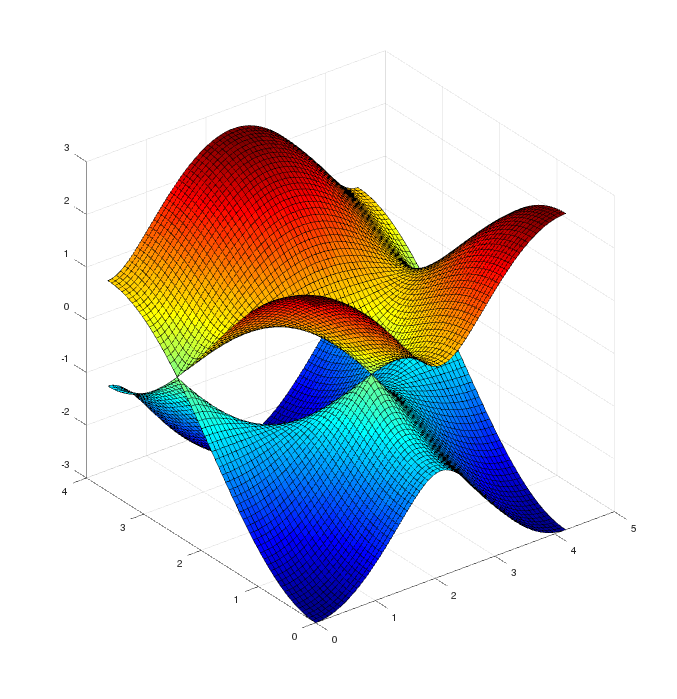
\includegraphics[scale=0.4]{graphics/specgraph.png}
\caption{Spectral bands of $H_{\textrm{km}}$ for $d = 1$ on the fundamental domain $[0,4\pi/3] \times [0,2\pi/\sqrt{3}]$ with $\lambda_{\textrm{nn}} = 1$ and $\lambda_{\textrm{se}} = \lambda_{\textrm{so}} = \lambda_{\textrm{ra}} = 0$}
\label{fig:specgraph}
\end{figure}
\item
   For $\lambda_{\textrm{nn}} \neq 0$, $\lambda_{\textrm{so}} \neq 0$ and $\lambda_{\textrm{ra}} = 0$ we can distinguish two topological phases: the ordinary insulator phase for $\lambda_{\textrm{se}} > 3\sqrt{3}\lambda_{\textrm{so}}$ (see figure \ref{fig:specins}) and the so called \textit{quantum spin hall (QSH)} phase for $\lambda_{\textrm{se}} < 3\sqrt{3}\lambda_{\textrm{so}}$ (see figure \ref{fig:specqsh}). Note that for $\lambda_{\textrm{ra}} = 0$ the third component of the spin is conserved and $H_{\textrm{km}}$ can be written as $H_{\textrm{km}}^{\uparrow} + H_{\textrm{km}}^{\downarrow}$. This means one Hamilton operator for each spin. Associated to each of them is an integer $n^{\uparrow},n^{\downarrow}$ which is the Chern number of $E_{P_{\textrm{km}}^{F}}$ for the according parts of the Hamilton operator as in section \ref{sec:topins}. And though $n^{\uparrow} + n^{\downarrow} = 0$ holds due to time reversal symmetry,
\begin{align*}
  \nu
  &:=
  \frac{n^{\uparrow} - n^{\downarrow}}{2}
  \in
  \mathbb{Z}
\end{align*}
isn't necessarily zero. In fact, according to \cite{f6db8935} we get
\begin{align*}
  I_{\textrm{km}}
  &=
  \nu
  \mod
  2
\end{align*}
In this case a conductance can occur. Namely if $n^{\uparrow} \neq 0$ there is a conductance of spin up electrons and consequently one of spin down electrons since the sum must be zero. This spin conductance is quantized. So one can speak of a \textit{quantized spin Hall\footnote{please note that the physical origin of this phenomenom is the magnetic field due to the spin-orbit coupling} conductance} for $\nu$.
\begin{figure}[H]
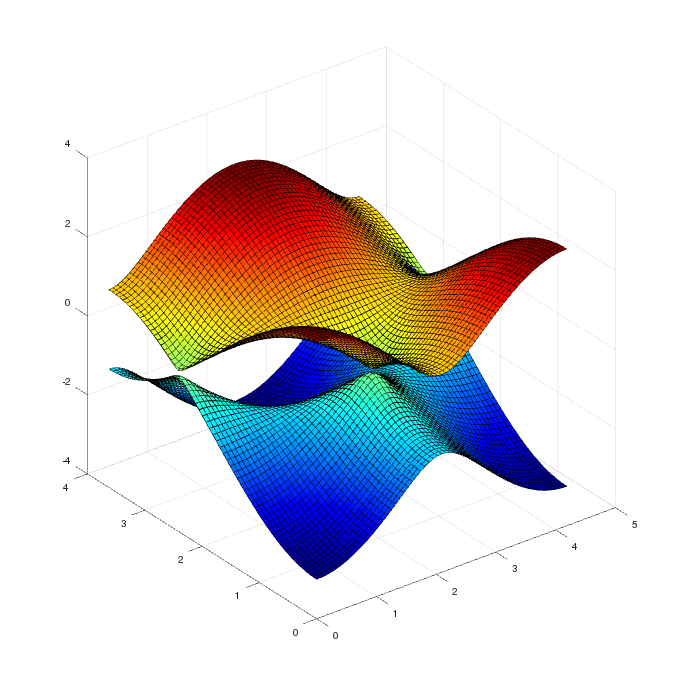
\includegraphics[scale=0.4]{graphics/specins.png}
\caption{Spectral bands of $H_{\textrm{km}}$ for $d = 1$ on the fundamental domain $[0,4\pi/3] \times [0,2\pi/\sqrt{3}]$ with $\lambda_{\textrm{nn}} = 1$, $\lambda_{\textrm{se}} = 0.1$, $\lambda_{\textrm{so}} = 0.006$ and $\lambda_{\textrm{ra}} = 0$}
\label{fig:specins}
\end{figure}
\begin{figure}[H]
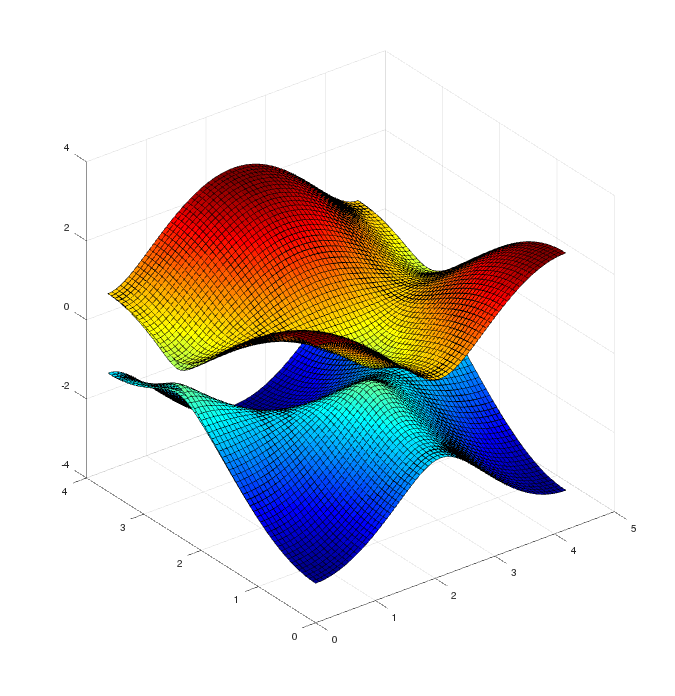
\includegraphics[scale=0.4]{graphics/specqsh.png}
\caption{Spectral bands of $H_{\textrm{km}}$ for $d = 1$ on the fundamental domain $[0,4\pi/3] \times [0,2\pi/\sqrt{3}]$ with $\lambda_{\textrm{nn}} = 1$, $\lambda_{\textrm{se}} = 0.1$, $\lambda_{\textrm{so}} = 0.06$ and $\lambda_{\textrm{ra}} = 0$}
\label{fig:specqsh}
\end{figure}
\item
  In the previous cases we assumed $\lambda_{\textrm{ra}} = 0$. But this is unrealistic and the unavoidably emerging rashba term kills the spin conservation. This makes $\nu$ meaningless. Nevertheless $I_{\textrm{km}}$ stays valid. There exists $x$ satisfying $x < 2\sqrt{3}\lambda_{\textrm{so}}$ such that QSH phase is retained for $0 \leq \lambda_{\textrm{ra}} \leq x$ if it was present for $\lambda_{\textrm{ra}} = 0$ (see figure \ref{fig:specrash}). If $x > 0$ there is still a spin conductance. However, it is not necessarily quantized anymore.
\begin{figure}[H]
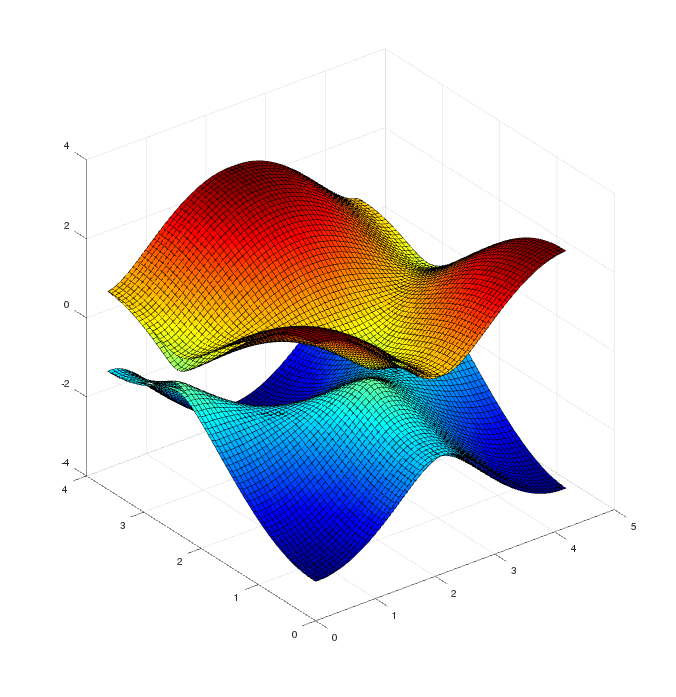
\includegraphics[scale=0.4]{graphics/specrash.png}
\caption{Spectral bands of $H_{\textrm{km}}$ for $d = 1$ on the fundamental domain $[0,4\pi/3] \times [0,2\pi/\sqrt{3}]$ with $\lambda_{\textrm{nn}} = 1$, $\lambda_{\textrm{se}} = 0.1$, $\lambda_{\textrm{so}} = 0.06$, $\lambda_{\textrm{ra}} = 0.05$}
\label{fig:specrash}
\end{figure}
\end{enumerate}
The Kane-Mele model is quite explicit. Indeed, it is explicit enough to implement it what we have done in \footnote{link to repo} and used in the above visualization of the energy bands. Another advantage of the implementation is to easily find propositions concerning the physiscs of the Kane-Mele model. Let us demonstrate in a concluding example on the thermodynamic pressure of the Kane-Mele model in an external magnetic field.
\\
\begin{exa}
\label{exa:tdpressure}
This example deals with a conjecture regarding a classical approximation of the Kane-Mele model's thermodynamic pressure in an external magnetic field on the basis of a numerical analysis.
\\
First, an external magnetic field in $e_{3}$ direction is described by the magnetic vector potential
\begin{align*}
  A(y_{1},y_{2})
  &:=
  (By_{2},0)
\end{align*}
for $B \in \mathbb{R}$. It can be incorporated into the Kane-Mele model by substituting the translation operators by so called \textit{magnetic translation}, that is, translation operators as above but with a position dependent \textit{phase $\exp(\mathrm{i}\phi_{i}(x))$}. To this end let $(x,0) := ((x_{1},x_{2}),0) \in \mathrm{C}_{\textrm{km}}$. Then $\gamma_{i}^{x}(t) = x +td_{i}$ for $t \in [0,1]$ and $i =1,2,3$ is a path connecting nearest neighbors and $\phi_{i}$ is given by
\begin{align*}
  \phi_{i}(x)
  =
  \int_{\gamma_{i}^{x}}
  (By_{2},0)
  \mathrm{d}y
  &=
  B
  \int_{0}^{1}
  (x_{2}+t(d_{i} \vert e_{2}),0)
  d_{i}
  \mathrm{d}t
  \\
  &=
  B
  (d_{i} \vert e_{1})
  \int_{0}^{1}
  (x_{2}+t(d_{i} \vert e_{2}))
  \mathrm{d}t
  =
  B
  (d_{i} \vert e_{1})
  x_{2}
  +
  \frac{1}{2}
  B
  (d_{i} \vert e_{1})
  (d_{i} \vert e_{2})
\end{align*}
So substrituting the explicit values for $d_{i}$ yields
\begin{align*}
  \phi_{1}(x)
  =
  \frac{dB}{2}
  x_{2}
  -
  \frac{\sqrt{3}d^{2}B}{8}
  &&
  \phi_{2}(x)
  =
  \frac{dB}{2}
  x_{2}
  +
  \frac{\sqrt{3}d^{2}B}{8}
  &&
  \phi_{3}(x)
  =
  -
  dBx_{2}
\end{align*}
and the magnetic translations $T_{d_{i}}^{B}$ are defined by
\begin{align*}
  T_{d_{i}}^{B}(\psi)(x)
  &:=
  \exp(\mathrm{i}\phi_{i}(x))
  T_{d_{i}}(\psi)(x)
\end{align*}
The numerics in \footnote{link to repo} suggest
\\
\begin{con}
\label{con:pressofkmm}
Let $B = B_{0} + \varepsilon b$ with $B_{0} \cdot \mathrm{vol}_{2}(\mathbb{R}^{2}/L_{\textrm{km}}) \in 2\pi\mathbb{Z}$, $b \in \mathbb{R}$ and $\varepsilon > 0$. Let further $\beta \in (0,\infty)$, $\mu = 0$ and $(\chi_{m})_{m\in\mathbb{N}^{\times}}$ such that $\chi_{m} \in \mathcal{S}(\mathbb{R}^{2},\mathbb{R})$ has support in $\Lambda_{m} \supset \mathrm{supp}(\chi_{m})$ with $\chi_{m} \vert \Lambda_{m-1} = 1$ if $\Lambda_{m} := [-m,m] \times [-m,m]$. Then the limit
\begin{align*}
  \lim_{\beta \to \infty}
  \beta^{-1}
  \lim_{m\to\infty}
  \frac{\varepsilon^{2}}{\Vert \chi_{m} \Vert_{L_{1}}}
  \mathrm{tr}_{\ell^{2}(\mathrm{C}_{\textrm{km}} \times \mathbb{C}^{2})}
  \left(
    \chi_{m}(\varepsilon x)
    \cdot
    \ln
    \left(
      1
      +
      \exp
      \left(
        -
        \beta
        \left(
          H_{\textrm{km}}^{B}
          -
          \mu
        \right)
      \right)
    \right)
  \right)
\end{align*}
exists and is approximated by
\begin{align*}
  \lim_{\beta \to \infty}
  \frac{1}{4 \cdot \mathrm{vol}_{2}(\mathbb{R}^{2}/L_{\textrm{km}}^{\prime})}
  \sum_{i=0}^{3}
  \int_{\mathbb{R}^{2}/L_{\textrm{km}}^{\prime}}
  \left(
    1
    +
    \varepsilon
    b
    \Omega_{(i)}
  \right)
  \ln
  \left(
    1
    +
    \exp
    \left(
      -
      \beta
      \left(
        h_{(i)}
        -
        \mu
      \right)
    \right)
  \right)
  \mathrm{d}k
  +
  \mathcal{O}(\varepsilon^{2})
\end{align*}
for $\varepsilon$ small enough where
\begin{align*}
  \Omega_{(i)}(k)
  &:=
  -
  \mathrm{i}
  \cdot
  \mathrm{tr}_{\mathbb{C}^{4}}
  \left(
    \tilde{P}_{\textrm{km}}^{\lbrace i \rbrace}(k)
    \left[
      \partial_{1}
      \tilde{P}_{\textrm{km}}^{\lbrace i \rbrace}(k),
      \partial_{2}
      \tilde{P}_{\textrm{km}}^{\lbrace i \rbrace}(k)
    \right]
  \right)
  \\
  h_{(i)}(k)
  &:=
  E_{i}(k)
  +
  \varepsilon
  b
  \cdot
  \mathrm{Im}
  \left(
    \mathrm{tr}_{\mathbb{C}^{4}}
    \left(
      \tilde{P}_{\textrm{km}}^{\lbrace i \rbrace}(k)
      \partial_{1}
      \tilde{P}_{\textrm{km}}^{\lbrace i \rbrace}(k)
      \left(
        \tilde{H}_{\textrm{km}}(k)
        -
        E_{i}(k)
        \cdot
        1_{\mathbb{C}^{4 \times 4}}
      \right)
      \partial_{2}
      \tilde{P}_{\textrm{km}}^{\lbrace i \rbrace}(k)
    \right)
  \right)
\end{align*}
\phantom{proven}
\hfill
$\square$
\end{con}
\phantom{proven}
\hfill
$\square$
\end{exa}
